% This is file JFM2esam.tex
% first release v1.0, 20th October 1996
%       release v1.01, 29th October 1996
%       release v1.1, 25th June 1997
%       release v2.0, 27th July 2004
%       release v3.0, 16th July 2014
%   (based on JFMsampl.tex v1.3 for LaTeX2.09)
% Copyright (C) 1996, 1997, 2014 Cambridge University Press

\documentclass{jfm}
\usepackage{graphicx}
\usepackage{epstopdf, epsfig}
\usepackage{amsmath}
\usepackage{amsfonts}
\newtheorem{lemma}{Lemma}
\newtheorem{corollary}{Corollary}

% our colors
\usepackage[usenames,dvipsnames]{xcolor}
\colorlet{cesar}{red}
\colorlet{greg}{green}
\colorlet{bill}{blue}

% copy-editing printing
% \usepackage{geometry}
% \geometry{a4paper,left=5.25cm,right=5 .25cm,top=3.5cm,bottom=3.5cm}
% \linespread{1.}
% \usepackage{multicol}


% our packages
%\usepackage{showlabels}

% hyperref
\usepackage{hyperref}
\hypersetup{
        %draft,
        breaklinks=true,
        colorlinks=true,
        linkcolor=blue,
        citecolor=Purple,
        urlcolor=Purple,
        pdfstartview={FitH},
        pdfview={FitH 0},
        pdfauthor={Cesar B. Rocha},
        pdftitle={stimulated generation},
 }


\newcommand{\NIW}{near-inertial wave}
\newcommand{\macrot}{macroturbulence}

%\shorttitle{ Extraction of  energy from barotropic turbulence by near-inertial waves}
\shorttitle{Stimulated generation}

\shortauthor{Cesar B. Rocha, Gregory L. Wagner, and William R Young}

%\title{Extraction of energy from quasi-gestrophic flow by near-inertial waves:\\
%        stimulated generation}
\title{Stimulated generation: extraction of energy from balanced flow
       by near-inertial waves}


%\title{Near-inertial waves extract energy from barotropic quasi-geostrophic flow}
\author{Cesar B. Rocha\aff{1}
  \corresp{\email{crocha@ucsd.edu}},
  Gregory L. Wagner\aff{2}
 \and William R. Young\aff{1}}

\affiliation{\aff{1}Scripps Institution of Oceanography, University of California,
            San Diego
\aff{2}Department of Earth, Atmospheric and Planetary Sciences, Massachusetts
            Institute of Technology}



\begin{document}

\include{symbols}

%\renewcommand{\sZ}{\mathsf{Z}}
%\renewcommand{\sE}{\mathsf{E}}
%\newcommand{\iBu}{\left(\tfrac{f_0}{N}\right)^2}
\newcommand{\F}{\mathcal{F}}
\newcommand{\D}{\mathcal{D}}
\newcommand{\phis}{\phi^\star}

%\newcommand{\bk}{\boldsymbol{k}}

\newcommand{\cg}{\mathbf{c}_g}
\newcommand{\Uf}{\mathbf{U}}
\renewcommand{\Im}{\mathrm{Im}}
\renewcommand{\div}{\nabla\cdot}
\renewcommand{\P}{\mathcal{P}}
\newcommand{\dU}{\delta U}
\newcommand{\W}{\mathcal{W}}
\newcommand{\cK}{\mathcal{K}}
\newcommand{\cP}{\mathcal{P}}
\renewcommand{\L}{\mathsf{L}}
\renewcommand{\N}{\mathsf{N}}
\newcommand{\psiq}{\psi^q}
\newcommand{\psiw}{\psi^w}
%\newcommand{\tfrac}{\frac}
%\newcommand{\eqref}{\ref}
\newcommand{\kb}{\mathbf{k}}
\newcommand{\xb}{\mathbf{x}}
%wave PV
\newcommand{\qw}{q^{\mathrm{w}}}
\newcommand{\bw}{b^{\mathrm{w}}}
\newcommand{\ug}{u^{\mathrm{g}}}
\newcommand{\bug}{\bu^{\mathrm{g}}}

%action and energy
\newcommand{\A}{  \mathcal{A}}
\newcommand{\E}{\mathcal{E}}
\newcommand{\Pw}{\mathcal{P}}
\newcommand{\Ke}{\mathcal{K}}
\newcommand{\Ff}{ \boldsymbol{\mathcal{F}}}
\newcommand{\Ffp}{\boldsymbol{\mathcal{F}}^{\perp}}
\newcommand{\Hf}{\boldsymbol{\mathcal{H}}}
\newcommand{\Gg}{\boldsymbol{\mathcal{G}}}
\newcommand{\epA}{\varepsilon_\mathcal{A}}
\newcommand{\epP}{\varepsilon_\mathcal{P}}
\newcommand{\epK}{\varepsilon_\mathcal{K}}

%dispersivity
\newcommand{\disp}{\eta}

%relative vorticity
\newcommand{\ze}{\zeta}

% index differentiation
\newcommand{\gind}[2]{#1_{,#2}}

% QG-NIW model (or XV model)
\newcommand{\coupledmodel}{QG-NIW model}


\maketitle

\begin{abstract}

Primitive-equation numerical simulations and analysis of reduced models suggest that stimulated
generation---the transfer of energy from
balanced flows to existing internal waves---is a leading contender for an ocean mesoscale
energy sink.  Here we study stimulated generation using an asymptotic model
that couples barotropic quasi-geostrophic flow and near-inertial waves with $\ee^{\ii m z}$ structure
on the $f$-plane.
 A detailed description of the conservation laws of this vertical plane-wave model illuminates
the mechanism of stimulated generation associated with vertical vorticity and lateral strain.
In particular, there are two sources of wave potential energy, and corresponding sinks of balanced
kinetic energy: (1) the refractive  convergence of the wave action density into anti-cyclones (and divergence from cyclones)
and (2)  enhancement of wave-field gradients by geostrophic straining.

We quantify the energy conversion and describe the phenomenology of stimulated
generation using numerical solutions of decaying ocean macroturbulence
modified by near-inertial waves. The initial conditions
are a uniform inertial oscillation and a two-dimensional turbulent field emergent from random
initial conditions. In all solutions, stimulated generation co-exists with a
 transfer of balanced kinetic energy to large scales, which is associated with vortex merger. And geostrophic straining
 accounts for most of the generation of wave potential energy, which represents a sink of 10-20\% of the initial balanced kinetic energy.
But refraction is fundamental  because it creates
the initial  eddy-scale lateral gradients in the near-inertial field that are then enhanced by
advection. In these quasi-inviscid solutions, wave dispersion is the only mechanism
that upsets stimulated generation: with barotropic balanced flow, lateral straining
enhances the wave group velocity; the waves accelerate and thus rapidly escape from the straining
regions. Because of this wave escape, the wave field does not suffer a direct cascade to dissipative scales.
\end{abstract}

\begin{keywords}

\end{keywords}


\section{Introduction}

% 1) The mesoscale energy conundrum: a recalcitrant problem
The  inverse cascade, acting on balanced ocean \macrot{},  transfers energy towards
large spatial scales. But a statistically steady ocean circulation requires
energy dissipation at the same rate as it is supplied  by wind.  Thus equilibration of
the  ocean \macrot{}  requires ageostrophic processes, acting in opposition to the
inverse cascade, to produce   a transfer of energy  towards the centimeter scales
at which molecular viscosity is effective.  Mechanisms that might result in this
down-scale transfer   include, but are not limited to, surface and
benthic boundary-layer turbulence, lee-wave generation by mesoscale eddies negotiating
bottom topography, and the spontaneous generation of internal waves by upper-ocean
frontal instabilities; see  \citet{nagai_etal2015} for a recent
review.

\begin{table}
\label{modelzTable}
\caption{Summary of model-based studies of energy extraction from balanced flow by near-inertial waves.}
  \begin{center}
     \begin{tabular}{ p{.285\textwidth} p{.4\textwidth} |   p{.3\textwidth}    }
     %\begin{tabular}{ c  p{.4\textwidth} l p{0.2\textwidth} }
       \hline
         Study &  Framework &   \textit{Stimulated generation} is referred to as \\ \hline
   \cite{gertz_straub2009} & {Barotropic 2D double-gyre solutions coupled with forced 3D
                              near-inertial waves.}
                              & \textit{2D--to--3D energy transfer}
                              \\ \hline
 \cite{thomas_2012} & {Near-inertial waves in a baroclinic geostrophic flow undergoing frontogenesis.}
                              & \textit{deformation shear production}
                              \\ \hline
    %\cite{whitt_thomas2015}  & Mixed-layer slab model modified by geostrophic
                              %relative vorticity.
                            %& \textit{geostrophic shear production}\\ \hline
     \cite{taylor_straub2016} & Boussinesq channel-flow with both  high- and
                                  low-frequency forcing.&
                                  \textit{advective sink}\\ \hline
    \cite{barkan_etal2016} & Boussinesq channel-flow  with both high- and
                                  low-frequency forcing.
                              & \textit{direct extraction}\\ \hline
    % \cite{jing_etal2017}  & Mixed-layer slab model modified by geostrophic
                              %relative vorticity and lateral strain.
                          %& \textit{}\\ \hline
    \cite{shakespeare_hogg2017} & Boussinesq channel-flow  with
                                  low-frequency forcing. Spontaneous generation in
                                  the surface layer and stimulated generation in
                                  the interior.
                                & \textit{interior amplification}
    \end{tabular}
  \end{center}
\end{table}


Here we focus on a mechanism first identified  by
\cite{gertz_straub2009}:  externally-forced \NIW s might provide an energy sink
for large-scale balanced flow. Since \cite{gertz_straub2009}, several other studies,
summarized in table \ref{modelzTable}, have argued for significant energy transfer
from balanced flows to \NIW s. A common aspect of the studies in table 1 is that
the  near-inertial waves are first introduced by  forcing at the inertial frequency  and then
grow by extracting energy from the balanced flow.

To distinguish this mechanism
from \textit{spontaneous} generation, and to complete an electromagnetic analogy,
 \citet{xie_vanneste2015} (XV hereafter) refer to the transfer of energy from balanced flow to externally forced near-inertial
waves  as  \textit{stimulated generation}.  The more widely studied process
of spontaneous generation is the emission of internal waves arising
from the slow evolution of balanced flow in the absence  of external forcing at
wave frequencies \citep{vanneste2013}. Spontaneous generation is inefficient at
small and  moderate Rossby numbers and its global impact on the energetics of the
ocean \macrot{}   is probably small \citep{danioux_etal2012, nagai_etal2015}.
Spontaneous generation is localized at sharp submeoscale fronts with  order-one
Rossby  number   \citep[e.g., ][]{shakespeare_hogg2017} while the stimulated variety  operates even at  small Rossby numbers characteristic of most interior oceanic conditions, provided only that internal waves are introduced by external forcing. Throughout the ocean, internal waves are reliably forced by wind and tides and thus stimulated generation is a leading contender as a mesoscale energy sink. Alternative terms to stimulated generation
used in the  literature are  summarized in  table \ref{modelzTable}.
The diversity of  studies in table \ref{modelzTable} indicates that stimulated
generation is a common, and therefore probably  important, wave mean flow interaction.

%( In the case of \citet{shakespeare_hogg2017},  near-inertial waves are produced in the high-Rossby number upper-ocean by  spontaneous generation and then propagate vertically  into the low-Rossby number deep-ocean interior, whereupon they  amplify by extraction of energy from balanced flow.)
 Using a variational formulation of the generalized Lagrangian mean, XV derived a  phase-averaged  model of the  coupling between near-inertial waves and quasi-geostrophic (QG) flow. \cite{wagner_young2016} derived a similar coupled model via Eulerian multiple-time expansion; these authors include the  second harmonic of the primary near-inertial wave  and simplify the wave dynamics by assuming  moderate QG vertical shears.  In both coupled models the near-inertial waves are governed by the equation of \cite{young_benjelloul1997} (YBJ hereafter) and the balanced flow satisfies QG dynamics---the waves contribute phase-averaged quadratic terms to the QG potential vorticity (PV). \cite{salmon2016} provides a useful perspective on these ``NIW-QG'' models; without assuming that the  waves are near-inertial, and within a single variational framework, Salmon unifies XV's model with the  wave-mean flow models of \cite{buhler_mcintyre1998} and  \cite{wagner_young2015}.

A central feature of the NIW-QG  model is that there are two integral energy conservation laws for  (1) near-inertial kinetic energy and (2) the sum of near-inertial potential energy and total balanced energy.
The NIW-QG model shows that stimulated generation is a consequence of the reduction in \NIW{} length scales
resulting from  advection and refraction of  waves by the balanced flow.  Reduction of wave length scales is accompanied by an increase in wave potential energy, and  because of conservation law (2), a reduction in the energy of the balanced flow.

Here we investigate perhaps the simplest example of stimulated generation obtained from  the NIW-QG model by assuming  barotropic QG flow and vertically-planar \NIW s.
Because
the balanced flow is barotropic, while the \NIW{} is three dimensional,
this ``vertical plane-wave model" resembles the original scenario of
\cite{gertz_straub2009}. We show that the convergence of wave kinetic energy
into anti-cyclones and  geostrophic straining of the  waves reduces the wave length
scale, amplifies  gradients of wave amplitude, and converts balanced kinetic
energy into near-inertial potential energy.

\section{The vertical plane-wave model}\label{TheModel}

The vertical plane wave model  is obtained by  assuming barotropic balanced flow, with streamfunction $\psi(x,y,t)$, a uniform background buoyancy frequency $N_0$,  and a single vertically propagating wave  with vertical structure $\ee^{\ii m z}$ and back-rotated wave velocity $\phi(x,y,t)$. With these idealizations,  appendix A derives the vertical plane-wave model  starting from the phase-averaged equations of  \cite{wagner_young2016};   XV obtain the same model from their version of the phase-averaged equations. In either case, the leading-order  velocity $(u,v,w)$, pressure $p$, and buoyancy $b$ are:
\begin{align}
\label{horizontal_velocity}
u + \ii v  &= \ee^{\ii \varpi}\,\phi -\psi_y + \ii\psi_x\,;\\
  \label{vertical_velocity}
  w &= \ii m^{-1}\ee^{\ii \varpi} \, \p  \phi  + \text{cc}  \,;\\
\label{pressure}
\qquad p &= - \ii \disp\ee^{\ii \varpi} \, \p \phi
+\text{cc} + f_0 \psi \,;\\
\label{buoyancy}
b &=  m \disp\ee^{\ii \varpi} \, \p \phi + \text{cc}
  \per
\end{align}
Above, $\varpi = m z - f_0 t $ is the  phase of the vertical plane wave,
$\disp = f_0\lambda^2$ is the wave ``dispersivity,'' where
$\lambda = {N_0}/{f_0\, m}$ is a  horizontal scale, cc denotes
complex conjugate, and
\beq
\p \defn \half (\p_x - \ii \p_y)
\eeq
is a differential operator. The complex field  $ \phi(x,y,t)$ in \eqref{horizontal_velocity}  is the  back-rotated velocity of the \NIW s;  in  \eqref{vertical_velocity}--\eqref{buoyancy} the  other wave fields   are  expressed in terms of  $\p \phi$. The compact representation of the wave variables in terms of  $\phi$ follows YBJ; the balanced variables are represented by the familiar QG streamfunction $\psi$.

%In other words, with $\psi=0$, \eqref{horizontal_velocity}--\eqref{buoyancy} are wave polarization relations.

The PV of the balanced flow is expressed in terms of $\psi$ and $\phi$ by \beq
\label{qgpv}
q = \underbrace{\lap \psi}_{\defn \ze} +
                 \underbrace{\tfrac{1}{f_0}\Big[ \tfrac{1}{4} \lap |\phi|^2 + \tfrac{\ii}{2}
                 \sJ(\phi^\star,\phi)\Big]}_{\defn \qw}\com
\eeq
where $\lap \defn \p_x^2 + \p_y^2$ is the horizontal
Laplacian and $\sJ(f,g) \defn f_x g_y - f_y g_x$ is the Jacobian, and
the superscript star $^\star$ denotes complex conjugation. Equation \eqref{qgpv}
is the ``inversion relation'': $q$ and $\phi$ determine the flow
as $\psi = \lap^{-1} (q - \qw) $ where $\qw$ defined in \eqref{qgpv} is the ``wave  potential vorticity.'' Once $\psi$ is obtained by inversion,
the field equations \eqref{macroturb} and \eqref{waves} below can be time-stepped.

Using the generalized  Lagrangian mean formulation \citet{buhler_mcintyre1998}
showed that the assumption of weak interaction between internal waves and balanced
flow results in wave-averaged terms contributing to the materially conserved
QGPV. In \eqref{qgpv} this wave-averaged
feedback on the balanced  flow is  expressed concisely in terms of the wave PV  $\qw$.

The balanced flow evolves according to  QGPV advection
\beq
\label{macroturb}
q_t + \sJ(\psi,q) = D_q\, ;
\eeq
the back-rotated velocity satisfies the  wave  equation
\beq
\label{waves}
\phi_t + \sJ(\psi,\phi) +  \phi \tfrac{\ii}{2}\ze - \tfrac{\ii}{2} \disp \lap \phi
 = D_\phi\per
\eeq
$D_q$ and $D_\phi$ in \eqref{macroturb} and \eqref{waves}  are dissipative terms
described below.

The wave equation \eqref{waves} is the YBJ  model in the
case where the \NIW{}  has $\ee^{\ii mz}$ structure. The back-rotated wave velocity, $\phi$,
evolves through dispersion---the last term on the left of  \eqref{waves}---and
nonlinear advection and refraction by the second and third terms in
\eqref{waves}.  Without advection, \eqref{waves} is analogous to Schr\"odinger's
equation \citep[e.g.,][ page 51]{landau_lifshitz2013}. The relative vorticity,
$\lap\psi$, is the potential, with negative $\lap \psi$ a  well, and the
``dispersivity,'' $\half f_0\lambda^2$, is Planck's constant \citep{balmforth1998, balmforth1999, danioux_etal2015}.
The quantum  analogy may be  useful for some readers, but it is not necessary for
the understanding of the results below.

The terms on the right of
\eqref{macroturb}  and \eqref{waves}, $D_q$ and $D_\phi$, represent small-scale
dissipation.  Small-scale dissipation is necessary to absorb the forward transfers
of potential enstrophy and wave kinetic and potential energies in the numerical
solutions reported below. We find that biharmonic diffusion and viscosity,
\beq\label{biharm}
D_q = -\kappa_e \lap^2 q\qquad\text{and}\qquad D_\phi = -\nu_\phi \lap^2 \phi\com
\eeq
are sufficient to extend the spectral resolution compared to Laplacian dissipation.
In practice, we choose $\kappa_e$ and $\nu_\phi$ so that  the highest 35$\%$
of the  modes lie in the dissipation range and aliased wavenumbers are strongly
damped.

%The
%\textit{ad hoc} introduction of these terms likely breaks the asymptotic ordering of the \cite{xie_vanneste2015}
%model.


\subsection{An illustrative solution: the Lamb-Chaplygin dipole}

\begin{figure}
\centering
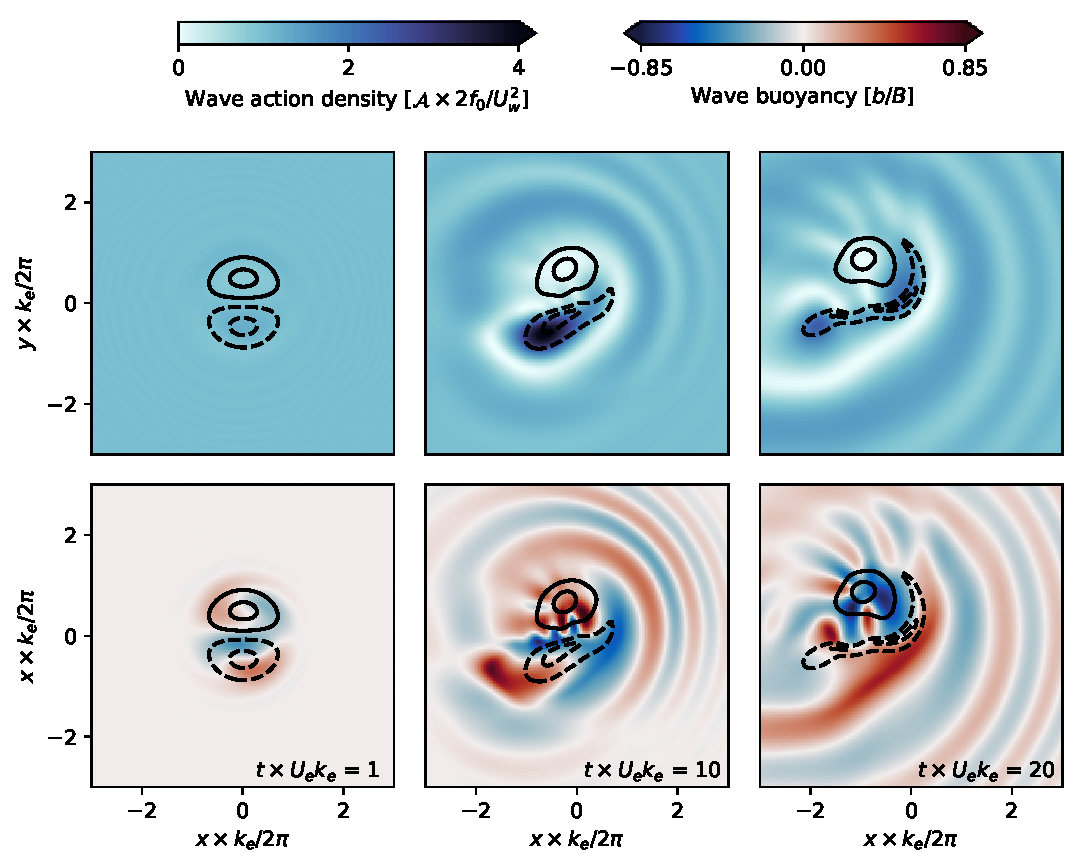
\includegraphics[width=.925\textwidth]{figs/fig1.png}
\caption{Snapshots of the Lamb-Chaplygin dipole solution with parameters presented
          in table \ref{parameters_lamb}.
        Contours depict potential vorticity, $q / (U_e k_e) = [
        -1.5,-0.5,0.5,1.5]$, with dashed lines showing negative values. The upper row shows the wave action density $|\phi|^2/2f_0$. The lower row shows the wave buoyancy;
        the buoyancy scale is $B = k_e m U_w f_0 \lambda^2$.
        These plots only show the central $(1/5)^2$
        of the simulation domain.}
        \label{snaps_lamb}
\end{figure}

\begin{table}
 \begin{center}
   \caption{Description of parameters of Lamb-Chaplygin simulation.
            The initial condition have Rossby number $Ro = U_e k_e/f_0 \approx
            0.05$, wave dispersivity $\hslash = f_0\lambda^2k_e/U_e
            \approx 1$, and wave amplitude $\alpha = Ro (U_w/Ue)^2 \approx 3.75$.}
   \label{parameters_lamb}
   \begin{tabular}{ l | l | l }
     \hline
      Parameter & Description & Value \\
      \hline
      $R= 2\pi k_e^{-1}$ & Dipole radius & $L_d/15 \approx 84$ km \\
      $U_e$ & Dipole strength & $5\times 10^{-2}$ m s$^{-1}$ \\
      $U_w$ & NIW speed & $5\times 10^{-1}$ m s$^{-1}$ \\
      $N_0$ & Buoyancy frequency & $5 \times 10^{-3}$ s$^{-1}$\\
      $f_0$ & Coriolis frequency & 10$^{-4}$ s$^{-1}$\\
      $2\pi$m$^{-1}$ & NIW vertical wavelength  & 325 m \\
      $\kappa_e$ & QGPV biharmonic diffusivity & $5\times 10^{7}$ m$^4$ s$^{-1}$\\
      $\nu_w$ & NIW biharmonic viscosity & $ 1 \times 10^{7}$ m$^4$ s$^{-1}$\\
      $\mathsf{N}$   & Number of modes &  512  \\
      $L_d$ & Domain size & $2\pi\times 200$ km \\
   \end{tabular}
 \end{center}
\end{table}


As a preamble to our discussion of stimulated generation  in freely-evolving
turbulence, we consider an example in which the initial QG flow
is the Lamb-Chaplygin dipole---see figure \ref{snaps_lamb}. This dipole is an
exact solution of the Euler equations on an infinite two-dimensional plane where
the vorticity is confined to a circle of radius $R$ \cite[][]{meleshko_vanheijst1994}.
The relative vorticity, steady in a frame moving at uniform zonal velocity $U_e$, is
\beq
\label{lambd_q}
  \ze =
     \frac{2 U_e \kappa}{J_0(\kappa R)} \begin{cases}
      J_1(\kappa r)\sin\theta\com & \text{if}
      \qquad r\le R\com\\
      0\com &\text{if} \qquad r\ge R\per
  \end{cases}
\eeq
Above $r^2 = (x-x_c)^2+(y-y_c)^2$ is the radial distance about the dipole's center
$(x_c,y_c)$, $\tan \theta = (y-y_c)/(x-x_c)$, and $J_n$ is the $n$'th order Bessel function. The matching condition at $r=R$ is that  $J_1(\kappa R)=0$ and the smallest solution is $\kappa R \approx
3.8317$.  If there is no coupling to the wave  $\phi$,  then the dipole \eqref{lambd_q} is a solution of the QG equation \eqref{macroturb}.

We strongly perturb the dipole in \eqref{lambd_q}  by seeding a wave  with initial velocity:
\beq
\label{NIO}
\phi(x,y,t=0) = \tfrac{1 + \ii}{\sqrt{2}}\, U_w\per
\eeq
If there was no dipole, this initial condition produces a spatially uniform  near-inertial oscillation with speed $U_w$.
Further parameters of this  solution are summarized in table  \ref{parameters_lamb}; note $U_w = 10 U_e$.



With the initial condition in \eqref{NIO},  $\qw $  in \eqref{qgpv}  and $\grad \phi$ are both  zero at $t=0$.
The refractive term in the wave equation  \eqref{waves}, however, immediately
imprints itself onto $\phi$ thus creating  non-zero $\grad \phi$ and non-zero
$\qw$.  Once refraction has created gradients
in $\phi$,  the advective term in \eqref{waves} can further distort $\phi$ and increase $\grad \phi$. This scale reduction of $\phi$ is most evident in the wave buoyancy shown in lower
row of figure \ref{snaps_lamb}. Figure \ref{snaps_lamb} also shows the well-known focussing  of waves into the negative vortex. But  the wave feedback on the mean flow through $\qw$ then results in distortion and shearing of the dipole so that the negative vortex loses its integrity;  the   lop-sided dipole then starts to drift. Once the negative vortex  is distorted to small scales it no longer acts as an effective potential well:  the trapping of wave energy by the deformed anti-cyclone  is weaker than in the initial condition. In fact, figure \ref{snaps_lamb}, which shows the  materially conserved PV $q$, understates the development of small scales in  the relative vorticity  $\ze$: figure \ref{squashed_bug} shows that both $\ze$ and $\qw$ develop small scales  with significant  cancelation  resulting in the relatively smooth field $q=\ze + \qw$ shown in figure \ref{snaps_lamb}. Thus at the final time in figure \ref{snaps_lamb} the waves are no longer strongly trapped  in the region with $\ze <0$. This phenomenology, including significant cancellation between $\ze$ and $\qw$, is also  characteristic of wave-modified two-dimensional turbulence in section \ref{turbulence}.

\begin{figure}
\centering
\includegraphics[width=.8\textwidth]{figs/fig1b.png}
\caption{(a) Snapshot of $q$ (contours) and $\zeta$ (colors) at $t \times U_ek_e=20$.
(b) Snapshot of $q$ (contours) and wave PV $\qw$ (colors). Both black lines
and colors depict the contour levels
$[ -1.5\, , -0.5\, , 0.5\, ,1.5] \times (U_e k_e)$. Solid lines and reddish colors depict
positive values; dashed lines and greenish colors show negative values. }
        \label{squashed_bug}
\end{figure}


 To understand the results in
figure \ref{snaps_lamb} and quantify the stimulated generation of wave energy,
we need to understand the  conservation laws of the vertical plane-wave model.


\section{Conservation laws of the vertical plane wave model}\label{physics}

XV noted that the vertical plane wave model in \eqref{qgpv} through \eqref{waves} inherits two quadratic conservation laws from the parent NIW-QG model: if there is no dissipation  then wave action,
\beq
\A \defn  \frac{|\phi|^2}{2 f_0} \com
\label{action}
\eeq
and the  energy,
\beq
\E \defn \half |\grad \psi |^2 + \quarter \lambda^2 |\grad \phi|^2  \com
\label{energy}
\eeq
are both separately  conserved.  Following \cite{BG1968}, the action in \eqref{action} is the wave energy divided by the intrinsic frequency; YBJ observed that to leading order the wave energy is only kinetic and   the intrinsic frequency in \eqref{action} is   the inertial frequency $f_0$.


 The conserved energy density $\E$ in \eqref{energy} is the sum of the kinetic energy of the balanced flow
\beq
\K\defn \half |\grad\psi|^2\com \label{EKE1}
\eeq
 and  the potential energy of the near-inertial waves,
\beq
\P \defn \half b^2 /N_0^2 = \quarter \lambda^2 |\grad \phi|^2 \per \label{potEnerg}
\eeq
Above, $b\propto \p\phi$ is the wave buoyancy defined in \eqref{buoyancy}. Because $\qw$ is quadratic in $\phi$ the conserved enstrophy,  $\la q^2 \ra$, is not a quadratic quantity.

XV explain the physical basis of stimulated generation by noting that balanced kinetic energy $\K$ can be converted into wave potential energy $\Pw$ while conserving  the integral of the total energy $\E$  in \eqref{energy}. Indeed, this conversion \textit{must} occur  if $\grad \phi$ is increased by a combination of refraction  and advection in the wave equation \eqref{waves}. In the example shown in  figure \ref{snaps_lamb}, the initial wave field in \eqref{NIO} has infinite spatial scale and therefore there is no  wave potential energy at $t=0$. The subsequent evolution  in figure \ref{snaps_lamb} involves creation of non-zero $\grad \phi$, corresponding to gain of $\Pw$ at the expense $\K$: this is  stimulated generation of near-inertial waves.

To substantiate this intuition, and diagnose results from our simulation of wave modified two-dimensional turbulence, we  develop the  conservation laws corresponding to \eqref{action} and \eqref{energy} in more detail.



\subsection{Action conservation equation  and action flux}

Multiplying the wave equation  \eqref{waves} by $\phis$ and adding to the complex conjugate we obtain a conservation equation  for action density
\beq
\label{action_density}
\p_t \A + \sJ(\psi,\A) + \diver \Ff =
\frac{\phis D_\phi + \phi D_{\phis}}{2 f_0}
\com
\eeq
where the flux of  \NIW{} action is
\beq
\label{Fw2}
\Ff \defn \tfrac{\ii}{4}\lambda^2 \left(\phi\grad\phis-\phis\grad\phi\right) \per
\eeq
The local conservation law  \eqref{action_density} shows how the wave action
$\A$ changes due to divergences of the geostrophic and wave fluxes and dissipation---the second, third, and fourth terms in \eqref{action_density}.



The wave action   flux $\Ff$ is analogous
to the probability current  of quantum mechanics
\citep[e.g., ][pg. 57]{landau_lifshitz2013}. Using the polar representation $\phi = |\phi|\ee^{\ii \Theta}$, the wave action  flux $\Ff$ can also be written as
\beq
\label{Fw2.1}
\Ff =  \A\,  \disp \grad\Theta \com
\eeq
where recall that $\disp = f_0\lambda^2$ is the dispersivity. In \eqref{Fw2.1},
$\disp \grad\Theta$ is the ``generalized group
velocity''  of hydrostatic \NIW s, i.e., $\Ff$ is the generalized group velocity times the action density $\A$. We use the term ``generalized'' because  no WKB-type  scale separation is required to obtain the  results above.  The connection to standard internal-wave group velocity is quickly verified by considering a plane near-inertial wave with  $\Theta = kx + ly$, yielding  $f_0\lambda^2\grad\Theta
= {N^2_0}(k,l)/{f_0 m^2}$.

Another useful identity involving the action flux  $\Ff$ is
\beq
\diver \big( \kay \cross \Ff \big)=\halfi \lambda^2 \sJ(\phis,\phi)\com  \label{uiden}
\eeq
where $\kay$ is the unit vector perpendicular to the $(x,y)$-plane. Using \eqref{uiden}, and the definition of action in \eqref{action}, the wave  PV $\qw$ in \eqref{qgpv} can be written as
\beq
\qw =  \half \lap \A +\eta^{-1}  \diver \big( \kay \cross \Ff \big)\per
\label{qwAlt}
\eeq

Denoting an average over the domain by $\la \ra$, and assuming that the action  flux divergence $\diver \Ff$ vanishes after integration, we obtain from \eqref{action_density}
\beq
\frac{\dd \la \A \ra}{\dd t} =\epA\ \per
\label{globAct}
\eeq
where $ \epA \defn \la\phis D_\phi + \phi D_{\phis} \ra/(2 f_0)$ is the domain average of the dissipative term on the right of \eqref{action_density}.
In the example shown in  Figure \ref{snaps_lamb} the total action $\la \A \ra$ is conserved to within $1$\% over the course of the integration.

\subsection{Ehrenfest's theorem}\label{eren}

The quantum analogy suggests that we should seek an analog of  Ehrenfest's theorem (the quantum equivalent of Newton's law that force equals mass times acceleration). Thus in  Appendix \ref{AppenB} we develop a local conservation law for $\Ff$. The domain average of that result is
\beq
\frac{\dd \la \Ff\ra}{\dd t} =  \kay \cross   \la \ze \, \Ff\ra    - \la  \A  \, \grad \half \ze  \ra   + \boldsymbol {\varepsilon}_{\Ff}\per
\label{Ehren}
\eeq
 In the quantum analogy, $\Ff$ is momentum and   the left hand side of \eqref{Ehren} is  mass times acceleration; the forces are on the right of \eqref{Ehren}. Starting from the end, $\boldsymbol {\varepsilon}_{\Ff}$ is a dissipative term defined in Appendix \ref{AppenB}. The second term on the right of \eqref{Ehren} is the force due to the gradient of the potential $\zeta/2$. The first term on the right of \eqref{Ehren} is a ``vortex  force,'' again  due to $\ze$, but perpendicular to $\Ff$; the vortex force lacks a quantum analog.

The results in this section are obtained from the wave
equation \eqref{waves} without using the  QGPV equation \eqref{macroturb}. In
other words, \eqref{action_density}-\eqref{Ehren} apply to the YBJ equation with $\ee^{\ii m z}$
structure regardless of the balanced-flow dynamics. We turn now to energy conservation and consideration of the QGPV equation   \eqref{macroturb}.

\subsection{Energy conservation and energy conversion}

The energy conservation law is considerably more complicated than action conservation.  We sequester the details of the local conservation laws to Appendix  \ref{AppenB} and present here the simpler results obtained by domain averaging those local conservation laws.
For the wave potential energy in \eqref{potEnerg} and the balanced kinetic energy in \eqref{EKE1} we find
 \begin{align}
 \frac{\dd \la \P \ra}{\dd t} &= \Gamma_{r} +\Gamma_a + \epP \com \label {ge1} \\
 \frac{\dd  \la \K \ra }{\dd t} &=
 - \Gamma_r - \Gamma_a + \Xi +  \epK \com \label{ge2}
 \end{align}
 where the ``conversion terms'' in \eqref{ge1} and \eqref{ge2}  are
 \begin{align}
 \Gamma_r &\defn  \Big\la\half\ze \, \diver\Ff \Big\ra\com \label{convr}
 \end{align}
 and
 \beq
  \Gamma_a \defn -\tfrac{\lambda^2}{2}
    \left\la
    \begin{bmatrix}
    \phi_x^\star & \phi_y^\star
    \end{bmatrix}
    \begin{bmatrix}
    -\psi_{xy} & \half(\psi_{xx} - \psi_{yy})\\
    \half(\psi_{xx}-\psi_{yy}) & \psi_{xy}
\end{bmatrix}
  \begin{bmatrix}
    \phi_x \\  \phi_y
    \end{bmatrix}\right\ra\per
    \label{conva}
\eeq
  The dissipative terms, $\epP$,  $\epK$ and $\Xi$  are defined in appendix \ref{AppenB}.  $\Xi$ in \eqref{ge2}  is particularly interesting: dissipation of waves $D_\phi$ produces balanced kinetic energy.
 Summing \eqref{ge1} and \eqref{ge2} the ``conversion'' terms $\Gamma_r$ and $\Gamma_a$  cancel, and we obtain the conservation law for total energy $\la \E \ra=\la \Pw + \K \ra$.

 %% dipole convergence figure %%
 \begin{figure}
 \centering
 \includegraphics[width=.92\textwidth]{figs/ConversionIllustration.png}
 \caption{Illustration of energy conversion terms in the Lamb-Chaplygin dipole solution
           with parameters presented
           in table \ref{parameters_lamb}. (a) The action  flux $\Ff$
           overlain on contours of relative vorticity $\lap\psi / (U_e k_e)
           = [-1.5,-0.5,0.5,1.5]$, with dashed lines showing negative values;
           the scale of the action flux is $F = f_0\lambda^2 k_e U_w^2$. (b) The
           local advective conversion
           (i.e., the unaveraged $\Gamma_a$) overlain on contours of streamfunction
           $\psi \times (U_e/k_e)= [-8,-4,-2,0,2,4,8]$.}
            \label{illustration_conversion}
 \end{figure}

\begin{figure}
\centering
\includegraphics[width=1.\textwidth]{figs/fig2.pdf}
\caption{Diagnostics of the Lamb-Chaplygin dipole solution with parameters presented
          in table \ref{parameters_lamb}. (a) Energy change about initial condition.
        (b) Wave potential energy budget \eqref{ge1}.
        }
        \label{stats_lamb}
\end{figure}



The refractive conversion  $\Gamma_r$   stems from $\ii \phi \ze /2 $  in the wave equation and is easy to
interpret: the convergence of the wave action  flux,
$\nabla\cdot\Ff < 0$, into anti-cylones, $\ze<0$, is a source of wave potential energy $\P$.
Figure \ref{illustration_conversion}a shows the convergence of $\Ff$ into the anti-cyclone
(and divergence from the cyclone) of the dipole solution at $t\times U_e k_e = 1$,
which yields the sharp initial increase of $\la \P \ra$ discussed below.
Ehrenfest's theorem in \eqref{Ehren} illuminates the initial structure of $\Ff$ in
figure \ref{illustration_conversion}. Because $\phi$ is initially uniform, the
initial tendency of $\la\Ff\ra$ is
\beq
\p_t \la\Ff\ra \approx -\disp \la\A \, \grad \half\ze\ra \per
\eeq
Thus, on average, the action flux is initially anti-parallel to the gradient of
relative vorticity; figure \ref{illustration_conversion} shows that in the dipole example  this result holds point-wise.

The  advective conversion $\Gamma_a$ in \eqref{ge1} and \eqref{ge2} stems from the term  $J(\psi,\phi)$ in the wave equation \eqref{waves} and is a source of $\la\Pw\ra$ due to straining and deformation of the wave field by the geostrophic flow. The symmetric $2\times 2$ matrix in \eqref{conva} is the strain or deformation tensor of the geostrophic flow. Thus, in analogy with passive scalar gradient amplification,   straining also enhances gradients
of the back-rotated near inertial velocity $\phi$, thereby generating wave potential energy $\la \P \ra$.


\subsection{Energetics of the Lamb-Chaplygin dipole solution}


Figure \ref{stats_lamb} shows the energetics of the Lamb-Chaplygin dipole
solution in  figure \ref{snaps_lamb}. In figure  \ref{stats_lamb}a, $\P$  increases at the expense of $\K$, while $\A$ is conserved. The wave potential energy budget in figure \ref{stats_lamb}b shows that
this stimulated generation occurs in two stages. First,
refraction of the initially uniform wave field causes a dramatic concentration
of waves into the anti-cyclone producing  a sharp increase $\P$ through
$\Gamma_r$. But this rapid initial energy conversion does not last long because
the wave feedback deforms the anti-cyclone and dispersion radiates
waves away from the dipole (see figure \ref{snaps_lamb}). Thus in figure \ref{stats_lamb}b,  $\Gamma_r$ decreases sharply, and eventually reverses sign at $t\times U_e k_e\approx 8$.

The second stage of stimulated generation in the dipole solution starts after
refraction has created dipole-scale waves. Advection by the balanced flow can then
strain the waves, further reducing their lateral scale (figure
\ref{stats_lamb}b). The ensuing advective conversion, $\Gamma_a$, starts
at $t\times U_e k_e \approx 4$. Straining by the balanced flow sustains this
advective generation of $\P$. The waves eventually
escapes the straining regions through dispersion and the conversion nearly halts at
$t\times U_e k_e = 30$.
The time-integrated $\Gamma_a$ accounts for $\approx 78\%$ of the
wave potential energy generation; table \ref{table1} summarizes  the energy budget.


% adds table 1, which is an output of a python script
% This is preferable, on reproducibility grounds, than adding values manually.
%\begin{table}
\begin{center}
    \caption{The time-integrated budget of wave potential energy and quasigeostrophic                kinetic energy of the Lamb-Chaplygin dipole solutions with parameters provided in table \ref{parameters_lamb}. The energy budgets close within $10^{-6}\,\%$.\label{table1}}
\begin{tabular}{c|c|c|c}
\hline
$\dot{P}_w$ budget & Fractional size ($\int\dot{P}_w \dd t/\Delta P_w $) & $\dot{K}_e$ budget  & Fractional size ($\int\dot{K}_e \dd t/\Delta K_e$)\\
\hline
$\Gamma_r$ & 0.228 & -$\Gamma_r$ & -0.227 \\
$\Gamma_a$ & 0.778 & -$\Gamma_a$ & -0.774 \\
$-$ & $-$ & $\Xi_r$ & 0.004 \\
$-$ & $-$ & $\Xi_a$ & 0.0 \\
$\chi_\phi$ & -0.006 & $\epsilon_\psi$ & -0.003 \\
Res. & 0.0 & Res. & 0.0 \\
\end{tabular}
\end{center}
\end{table}

\begin{table}
\begin{center}
    \caption{The time-integrated budget of wave potential energy and quasigeostrophic      kinetic energy of the Lamb-Chaplygin dipole solutions with parameters provided in table \ref{parameters_lamb}. The energy budgets close within $10^{-6}\,\%$.\label{table1}}
\begin{tabular}{c|c|c|c}
\hline
$\dot{P}_w$ budget & Fractional size ($\int\dot{P}_w \dd t/\Delta P_w $) & $\dot{K}_e$ budget  & Fractional size ($\int\dot{K}_e \dd t/\Delta K_e$)\\
\hline
$\Gamma_r$ & 0.228 & -$\Gamma_r$ & -0.227 \\
$\Gamma_a$ & 0.778 & -$\Gamma_a$ & -0.774 \\
$-$ & $-$ & $\Xi_r$ & 0.004 \\
$-$ & $-$ & $\Xi_a$ & 0.0 \\
$\chi_\phi$ & -0.006 & $\epsilon_\psi$ & -0.003 \\
Res. & 0.0 & Res. & 0.0 \\
\end{tabular}
\end{center}
\end{table}


\subsection{Summary}

The  expressions for energy conversion in \eqref{convr} and \eqref{conva} clarify the mechanism of stimulated generation triggered by  the initially uniform \NIW{} in \eqref{NIO}. First, refraction causes a convergence of wave action  into anti-cyclones. Then advection strains the waves, reducing their lateral scale. Both
processes amplify the lateral gradients of wave amplitude, thereby generating wave potential energy $\Pw$ at the expense of balanced kinetic energy $\K$. Wave action $\A$ is conserved throughout this process.

In the remainder of this paper, we describe and quantify  stimulated generation in an idealization of an oceanographic post-storm scenario:  the  uniform initial  \NIW{} in \eqref{NIO} interacts with two-dimensional  turbulence.




\section{Macroturbulence modified by \NIW s}\label{turbulence}

To study the energy exchange between near-inertial geostrophic flow
in an oceanographic turbulent regime, we consider a barotropic flow that emerges from
random initial conditions integrated for 20 eddy turnover time units.
In other words, we first integrate the initial condition
\beq
\label{psi_init}
\psi \big(x,y, t \times U_e k_e = -20\big) = \sum_{k,l} \psi_\kb \cos\left(k x + l y +
\chi_\kb\right)
\eeq
with waveless QG dynamics before introducing the wave in \eqref{NIO} at $t\times U_e k_e = 0$.
Above, $\chi_\kb$ is a random phase uniformly distributed on $[0, 2\pi)$,
 and $\psi_\kb$ is the streamfunction isotropic spectrum
\beq
\label{psih_mag}
\psi_\kb = C \times \big\{|\kb|\,[1 + (|\kb|/k_e)^4]\big\}^{-1/2}\com
\eeq
with the wavenumber magnitude $|\kb|^2 = k^2 + l^2$. The prescribed initial energy
$U_e^2/2$ determines the constant $C$:
\beq
\label{ke_init}
\sum_{k,l} \underbrace{|\kb|^2 {\psi_\kb}^2}_{\defn \cK_e} = \tfrac{1}{2}U_e^2\per
\eeq
The kinetic energy spectrum, $\cK_e$, peaks at the energy-containing scale $k_e^{-1}$.
At scales larger than $k_e^{-1}$, $\cK_e$ has a linear dependence on $|\kb|$,
whereas $\cK_e$ decays as $|\kb|^{-3}$ at scales smaller than $k_e^{-1}$. This red spectrum
ensures insignificant loss of energy by small-scale dissipation $D_q$ in \eqref{macroturb}.

%   $$
%  \hat \psi_{\kb} =  \frac{C}{\sqrt{|\kb| [1 +( |\kb|/k_e)^4]}}
% $$
%  I don't see why it is necessary to put $| \ |$ around $ \hat \psi_{\kb} $? It is defined so that it is real and positive.}

 The evolution of a random initial condition under quasi-inviscid
QG dynamics \eqref{macroturb} has been well studied, beginning perhaps
with \cite{fornberg1977}.
  Stirring of vorticity $\lap \psi$ transfers enstrophy towards
 small scales; energy flows to large
 scales. Most of enstrophy is dissipated within few eddy turnover times, whereas
 kinetic energy is nearly conserved. Vorticity concentrates into localized coherent
 structures: after 20 eddy turnover time units, the vorticity is well-organized
 into an ensemble of vortices that form via like-sign vortex merging
 \citep[e.g., ][]{mcwilliams1984}.



% We add a uniform near-inertial oscillation \eqref{NIO} to the mature
% barotropic turbulence at $t \times U_e k_e = 0$.
 % \textcolor{red}{For all parameters considered
 % in the remainder of the paper, there are no qualitative long-term differences
 % between the solutions described below and results from introducing the waves
 % at $t\times U_e k_e = -20$.}
 % \centerline{\textcolor{bill}{Why say the red stuff  above?}}

 \subsection{Relevant parameters}
The scaling
 \begin{align}\label{scaling}
    \text{length}    \sim  k_e^{^{-1}}\com\qquad
    \text{time}    \sim (U_e k_e)^{-1}\com\qquad
    \psi \sim U_e k_e^{-1} \com
    \text{and}\qquad\phi \sim U_w\com
 \end{align}
 shows that there are two important dimensionless control parameters. The first is
  \beq
 \label{alpha}
 \alpha \defn \underbrace{\frac{U_e k_e}{f_0}}_{\defn Ro} \times
 {\left(\frac{U_w}{U_e}\right)^2}\com
 \eeq
 which measures the strength of the waves compared to the geostrophic flow and scales
 the contribution of the wave terms in the potential vorticity \eqref{qgpv}.
The second dimensionless parameter is
 \beq
 \label{hslash}
 \hslash \defn \disp \times \frac{k_e}{U_e}\com
 \eeq
which  scales wave dispersion against the   effects of advection and refraction.

 \begin{table}
  \begin{center}
    \caption{Description of parameters of the macroturbulence simulations.
             The initial condition have Rossby number $Ro = U_e k_e/f_0 \approx
             0.05$, wave dispersivity $\hslash = f_0\lambda^2k_e/U_e
             \approx 0.5-2$, and wave amplitude $\alpha = Ro (U_w/Ue)^2 \approx 0.2$.}
    \label{parameters_turb}
    \begin{tabular}{ l | l | l }
      \hline
       Parameter & Description & Value \\
       \hline
       $R= 2\pi k_e^{-1}$ & Energy-containing scale & $L_d/10 \approx 125$ km \\
       $U_e$ & Eddy velocity & $5\times 10^{-2}$ m s$^{-1}$ \\
       $U_w$ & NIW speed & $1 \times 10^{-1}$ m s$^{-1}$ \\
       $N_0$ & Buoyancy frequency & $5 \times 10^{-3}$ s$^{-1}$\\
       $f_0$ & Colioris frequency & 10$^{-4}$ s$^{-1}$\\
       $2\pi$m$^{-1}$ & NIW vertical wavelength & $280-560$m \\
       $\kappa_e$ & QGPV biharmonic diffusivity & $5\times 10^{6}$ m$^4$ s$^{-1}$\\
       $\nu_w$ & NIW biharmonic viscosity & $ 5 \times 10^{6}$ m$^4$ s$^{-1}$\\
       $\mathsf{N}$   & Number of modes &  1024  \\
       $L_d$ & Domain size & $2\pi\times 200$ km \\
    \end{tabular}
  \end{center}
 \end{table}

 \begin{figure}

 \centering
 \includegraphics[width=1.\textwidth]{figs/fig3.png}
 \caption{Snapshots of the  turbulence solution with parameters  in
          table \ref{parameters_turb}. Upper panels: QGPV. Middle panels: wave kinetic energy  density $|\phi|^2$.
         Bottom panels: wave buoyancy, with scale  $B = k_e m U_w f_0 \lambda^2$.
        These plots  show
        $(1/2)^2$ of the  domain.}
         \label{snaps_turb}
 \end{figure}

 \begin{figure}
 \centering
 \includegraphics[width=1.\textwidth]{figs/fig4.pdf}
 \caption{Diagnostics of the macroturbulence solution with parameters presented
           in table \ref{parameters_turb}. (a) Energy change about initial condition.
         (b) Wave potential energy budget \eqref{ge1}.
         }  \label{stats_turb}
 \end{figure}


 \begin{table}
 \begin{center}
     \caption{The time-integrated budget of wave potential energy and QG
              kinetic energy of the reference macroturbulence solution with
              parameters in \ref{parameters_turb}. The energy budgets close
              within $0.1\,\%$.\label{table2}}
 \begin{tabular}{c|c|c|c}
 \hline
 $\dot{P}_w$ budget & Fractional size ($\int\dot{P}_w \dd t/\Delta P_w $) & $\dot{K}_e$ budget  & Fractional size ($\int\dot{K}_e \dd t/\Delta K_e$)\\
 \hline
 $\Gamma_r$ & 0.117 & -$\Gamma_r$ & -0.108 \\
 $\Gamma_a$ & 0.907 & -$\Gamma_a$ & -0.839 \\
 $-$ & $-$ & $\Xi_r$ & 0.009 \\
 $-$ & $-$ & $\Xi_a$ & 0.003 \\
 $\chi_\phi$ & -0.026 & $\epsilon_\psi$ & -0.062 \\
 Res. & 0.003 & Res. & 0.003 \\
 \end{tabular}
 \end{center}
 \end{table}


\subsection{Solution with $\hslash = 1$ and $\alpha = 0.1$}

% General remarks about the flow evolution
Figure \ref{snaps_turb} show snapshots of a solution with
$\hslash = 1$ and $\alpha = 0.1$ and further parameters in table \ref{parameters_turb}.
This turbulence solution shares qualitative aspects of the Lamb-Chaplygin solution.
Starting from a uniform wave field in \eqref{NIO}, refraction quickly concentrates the waves into
anti-cyclones. By
$t\times U_e k_e \approx 1$ there is a two-fold modulation of the wave action
density on eddy scales with significant focussing of waves in anti-cyclones
(compare middle and upper panels of figure \ref{snaps_turb}).

Dispersion radiates waves from the vortices; advection enhances
the gradients of  back-rotated velocity $\phi$  (see lower panels of figure \ref{snaps_turb},
which depict wave buoyancy). By $t\times U_e k_e \approx 10$ there is a five-fold
modulation of the wave kinetic energy density and the wave buoyancy has been
amplified by a factor of two. The evolution of  potential vorticity $q$ is  similar to  that in the
waveless problem: like-sign vortices merge into bigger vortices. The big vortices keep straining the waves, generating smaller  scales in the wave field.

% The energetics
Figure \ref{stats_turb}a shows the inexorable increase in wave potential energy $\la \P\ra$ and the corresponding decrease in balanced kinetic energy $\la \K \ra$. In figure \ref{stats_turb}b quick wave refraction results in an  initial sharp generation of $\la \P\ra$  at the expense of balanced kinetic energy $\la \K\ra$.  As in the Lamb-Chaplygin solution, the positive refractive
conversion, $\Gamma_r > 0$, is ephemeral: in figure \ref{stats_turb}b, $\Gamma_r$  peaks at $t\times U_e k_e \approx 2$ and then decays
rapidly, eventually changing sign at $t\times U_e k_e \approx 5$.
But a significant positive advective conversion, $\Gamma_a> 0$, sustains  stimulated generation so that  $\la \P\ra$
ultimately increases approximately linearly with time.

After 25 eddy-turnover time units, the balanced kinetic energy $\la \K\ra$ has decayed by about
$14 \%$ from its  initial value. Most of this loss  is
by  stimulated generation of $\la \P\ra$. As in the Lamb-Chaplygin solution,
advective conversion accounts for most of the energy change. Table \ref{table2}
presents further details of the energy budget.

% Now discuss the main features
The solution illustrates  interesting characteristics of  stimulated generation. First, the role of refraction is catalytic in that it generates the initial eddy-scale gradients in  $\phi$
that are then enhanced by advective straining; the advective conversion, $\Gamma_a$ in \eqref{conva}, ultimately  accounts for most of the energy transfer from turbulence  to waves. Second, the roughly linear--in--time growth of  wave potential energy $\la \P\ra$ is very slow in comparison with exponential increase of  passive-scalar tracer gradients in turbulent velocity fields. The relatively  slow
growth  of $\la \P\ra$ suggests that wave dispersion plays an important role in slowing and perhaps opposing
advective straining (see section \ref{discussion} for further discussion of dispersion and ``wave escape''). To investigate whether these characteristics are general we consider
solution with varying vertical wavelengths and therefore different dispersivities.

\subsection{Varying dispersivity \label{dummy}}

 \begin{figure}
 \centering
 \includegraphics[width=1.\textwidth]{figs/fig5.png}
 \caption{Snapshots of QGPV $q$ and its
          decomposition into relative vorticity $\ze = \lap\psi$, and wave
          potential vorticity $\qw$. The snapshots were taken at $t\times U_e k_e =25$.
         }  \label{pv-terms_turb}
 \end{figure}

Figure \ref{pv-terms_turb} shows snapshots of potential vorticity $q$ and its constituents  in a set of solutions with varying the vertical wavelength
$2\pi\,m^{-1}$ from 280 to 560 m, yielding dispersivities ranging from 0.5 to 2.
(All other parameters are fixed.) The potential vorticity $q$ shows more small-scale
filamentation with decreasing dispersivity, but it is otherwise remarkably similar across
the three solutions. The partition into relative vorticity $\lap\psi$ and wave potential
vorticity $\qw$, however, depends significantly on dispersivity. In particular,
$\qw$ develops smaller scales and larger amplitudes with decreasing dispersivity.
As anticipated by the dipole example in figure \ref{squashed_bug}, there is  cancellation of small-scale features in $\qw$ against those in  $\ze$ so that  $q$ is relatively smooth even in the solution with  weak dispersion $\hslash=0.5$.


\begin{figure}
\centering
\includegraphics[width=1.\textwidth]{figs/fig6.pdf}
\caption{The energetics of macroturbulence solutions with different
         dispersivities. (a) Energy change about the initial condition.
         (b) The energy conversion terms in \eqref{ge1}.
        } \label{stats_turb_various}
\end{figure}

\begin{figure}
\centering
\includegraphics[width=1.\textwidth]{figs/fig7.pdf}
\caption{Diagnostics of macroturbulence solutions with different
         dispersivities. (a) The correlation between relative vorticity and
         wave kinetic energy. (b) The skewness of relative vorticity.
        } \label{correlation_skewness}
\end{figure}


The initial evolution of the uniform wave field is similar across dispersivities,
with refraction initially  generating eddy-scale gradients of the waves---see figure \ref{stats_turb_various}.
Refraction produces a sharp initial increase of wave potential energy and decrease
of balanced kinetic energy, which is almost independent of dispersivity. Figure \ref{correlation_skewness}a
shows  that this initial
``refractive stage'' yields a strongly negative wave-vorticity correlation $r$,
\beq
r \defn \frac{\la \zeta \A' \ra}{\sqrt{\la\zeta^2\ra\la\A'^2\ra}}\com
\label{rdefn}
\eeq
where $\A'\defn (|\phi|^2-|\la\phi\ra|^2)/f_0$; in figure \ref{correlation_skewness}a the initial negative $r$
is nearly independent of dispersivity. Because significant energy exchange
takes place in the anti-cyclones due to the initial wave concentration, a positive
vorticity skewness ensues (figure \ref{correlation_skewness}b). Once the
eddy-scales are created, advection strains the waves and  generates further  wave
potential energy at the expense of balanced kinetic energy. It is in this stage
that the dependence on dispersivity is pronounced: weakly dispersive waves are
strained further than strongly dispersive waves. Thus the advective conversion becomes
stronger with decreasing dispersivity (figure \ref{stats_turb_various}b). Advection
and dispersion significantly reduces the wave-vorticity correlation; the reduction
in correlation increases as the dispersivity decreases (figure \ref{correlation_skewness}a). For the weakest dispersivity
considered, the wave-vorticity correlation becomes weakly positive likely because of
the initial positive vorticity skewness.

\begin{figure}
\centering
\includegraphics[width=1.\textwidth]{figs/FigSpectraVarious.pdf}
\caption{Energy-preserving spectra of macroturbulence solutions with different
         dispersivities. The three panels show spectra of (a)  balanced kinetic energy
          $\K$ , (b) wave action $\A$, and (c) wave potential
          energy $\P$. All solid lines correspond to spectra at
          $t\times U_e k_e = 25$ and the dashed line in (a)  is
          the balanced kinetic energy spectrum at $t\times U_ek_e = 0$.
        } \label{spectra_turb_various}
\end{figure}

In all solutions reported above, the evolution of the balanced flow  is similar  to that of
waveless  macroturbulence:
there is a transfer of balanced energy towards larger scales driven by merger of  like-signed
vortices---see figure \ref{spectra_turb_various}a. The main difference is that
balanced kinetic energy is not conserved; kinetic energy is constantly transformed
into wave potential energy via stimulated generation. The stimulated generation process
is associated with a forward transfer of wave action $\A$ from the infinite horizontal
scale in the initial condition \eqref{NIO}  to the eddy scale; see figure \ref{spectra_turb_various}b. The wave potential
energy density $\P$ in figure \ref{spectra_turb_various}c develops significantly smaller scales  than those of the balanced
kinetic energy $\K$ in figure \ref{spectra_turb_various}a.

\section{Discussion and conclusions}\label{discussion}
The  expression for the energy conversion in \eqref{ge1} illuminates the
physics of stimulated generation: both convergence of wave action density
into anti-cyclones \eqref{convr} and geostrophic straining of the wave field \eqref{conva} are sources of wave potential
energy and sinks of balanced  kinetic energy. But this characterization
of stimulated generation ignores the important role of wave dispersion---waves can
propagate out of the vorticity or straining regions, thereby reducing the
correlations $\Gamma_r$ and $\Gamma_a$ required for stimulated generation.

\begin{figure}
\centering
\includegraphics[width=1.\textwidth]{figs/figesc.png}
\caption{A comparison of passive-scalar and wave solutions ($\hslash \approx 0.09$)
          with
          same initial conditions (the wave kinetic energy is equal
          the passive-scalar variance) and same small-scale dissipation.
          (a) Initial condition of wave back-rotated zonal velocity and  of the passive scalar.
          (b) Wave back-rotated zonal velocity at $t\times U_e k_e = 10$. (c)
          Passive-scalar concentration at $t\times U_e k_e = 10$. (d) Variance
          of wave velocity or passive-scalar variance. (d) Variance of wave velocity gradient or
          passive scalar. In (d) and (e),
          the diagnostics are normalized by their initial values.
        } \label{wave_escaping}
\end{figure}

\subsection{Wave escape  }
Wave dispersion is indeed the only mechanism that upsets stimulated generation
in the quasi-inviscid solutions described in this paper. In all solutions, after
an initial conversion due to refraction,
advective straining accounts for most of the energy conversion. Experience with the passive-scalar problem suggests (incorrectly) that the wave potential energy  $\P$ should then increase exponentially with time as $\grad \phi$ is amplified by stirring  \citep[e.g., ][]{YRG1982}. But even in the
weakly dispersive limit, the waves do not behave as a passive scalar (see figure \ref{stats_turb_various}) and stimulated generation is much less effective than suggested by this ``passive-scalar thinking.'' This is
because advective  straining can only increase $\grad \phi$ so much:
the near-inertial generalized group velocity is $\disp\grad\Theta$
(cf. section \ref{physics}), where $\Theta$ is the phase of the near-inertial
back-rotated velocity $\phi = |\phi|\ee^{\ii\Theta}$. Geostrophic straining enhances  $\grad\Theta$
thereby increasing the near-inertial group velocity so that the waves escape the straining
region. Thus, straining by a barotropic balanced flow results in  near-inertial ``wave escape,''
as opposed to the  ``wave capture'' described by \citet{buhler_mcintyre2005}. Indeed, wave capture requires \textit{both}
lateral strain \textit{and} vertical shear: the  vertical plane wave model has no vertical shear and therefore wave capture is inoperative;  see \citet[][]{thomas_2012} for further discussion of the importance of vertical shear to wave capture.

We are surprised by the successful resistance mounted  by the waves  to strain-driven exponential amplification of $\grad \phi$    and thus seek to illustrate wave escape with a simple flow. Figure \ref{wave_escaping} shows the escape of a wave packet initially
placed at the saddle point of a large-scale balanced flow with  $\psi \propto \sin x + \sin y$. The behavior
of the wave packet is qualitatively different from that of a  passive scalar in the same flow. The passive scalar
packet is strained until it is diffused into oblivion. On the other hand,  the waves are strained just so much, resulting in acceleration and escape from  the straining region; the waves finally  concentrate in the regions with non-zero vorticity, i.e., in the regions where the  Okubo-Weiss criterion indicates no exponential stretching.
The top row of figure \ref{wave_escaping} depicts this striking difference between the behavior of passive scalar and waves. In the bottom row, figure \ref{wave_escaping}d shows that
while wave action $\propto |\phi|^2$ is nearly conserved, the analogous passive-scalar variance is nearly fully dissipated. Figure \ref{wave_escaping}e shows that the variance of the passive-scalar gradient at first  increases
exponentially due to straining and then decays  due to diffusion. On the other hand,   the potential energy of the waves $\propto |\grad \phi|^2$ increases slowly and then oscillates around an equilibrium level. The wave-escape phenomenology in the  turbulence solutions of section \ref{turbulence} qualitatively resembles that seen in this simple flow. In particular,  the wave potential energy does not reach the dissipative scale (figure \ref{spectra_turb_various}c).

\subsection{Absence of a direct cascade of wave energy }

The solutions reported here  introduce the waves at $t=0$ in \eqref{NIO} with infinite spatial scale. Wave refraction, $\ii  \phi \zeta/2$ in \eqref{waves}, immediately transfers  wave energy to  the smaller scales of the balanced relative vorticity $\zeta$. This giant leap across wavenumbers  is not a direct cascade of  wave energy in the sense of Kolmogorov. In fact,   because of wave escape,  the wave energy that is efficiently transferred to  eddy scales by refraction does not suffer a turbulence-driven direct cascade to the small length scales at which the  dissipation  \eqref{biharm} is effective. This conclusion hinges on the assumption of a barotropic balanced flow: there still remains the possibility of a direct cascade of wave energy if the balanced flow has vertical shear. If the waves can be coerced into a direct-cascade to small scales then stimulated generation would be stronger than in  the vertical plane-wave model.

\subsection{Regimes of wave-modified turbulence}
Geostrophic straining accounts for most of the stimulated generation of wave energy
in the examples considered in this paper. But refraction plays a fundamental role
in these solutions with the  uniform (laterally coherent) initial wave velocity in \eqref{NIO} because
refraction creates the initial gradients of wave velocity that are then enhanced
by geostrophic straining.  We experimented by changing the initial condition of $\phi$ to
an eddy-scale plane wave and repeated all the macroturbulence solutions; the different initial condition  significantly suppresses the initial refraction stage, but otherwise yields
long-term solutions that are qualitatively similar to the solutions discussed above.
Thus, to the extent that the uniform-wave initial condition  \eqref{NIO} idealizes the
generation of large-scale upper-ocean inertial oscillations by storms
\citep[e.g., ][]{moehlis_llewellynsmith2001,danioux_etal2015}, the initial refraction
is  a loss of lateral coherence, or a type of inertial pumping
\citep{young_benjelloul1997,klein_etal2004}, which
is accompanied by an extraction of energy from the balanced flow by the waves.

Although 10-20\% of the
balanced kinetic energy is converted into wave potential energy, and despite the wave breakage of the symmetry between  cyclones and anti-cyclones, the wave-modified turbulence in section \ref{turbulence} remarkably resembles waveless two-dimensional turbulence  \citep[e.g., ][]{mcwilliams1984}: we still observe robust vortices and an increase in vortex length scale   due to  merger of like-signed vortices. Figure \ref{pv-terms_turb} shows  small changes in the potential vorticity $q$  and much  larger changes in the wave PV $\qw$ induced by changing the dispersivity. In this sense, the turbulent evolution is  insensitive to wave modification.

To see significant wave modification of the turbulence we increased the amplitude of the  initial wave in \eqref{NIO} so that  $U_w = 6 U_e$ (in section \ref{turbulence}, $U_w=2 U_e$).  With this level of wave energy the wave-modified macroturbulence differs qualitatively from the waveless variety (not shown). The potential vorticity develops highly filamentary structures with little vortex formation; this inhibition of vortex formation is  stronger
in the weakly dispersive limit. But this large amplitude, weakly dispersive case is probably irrelevant to ocean dynamics.


\subsection{The correlation of wave amplitude with  relative vorticity}

A secondary result here
is the strong time-dependence of the correlation $r$, defined  in \eqref{rdefn}, between incoherent waves and
the relative vorticity; $r$ measures the concentration of waves into cyclones or
anti-cylones \citep{danioux_etal2015}. Refraction concentrates  waves into anti-cylones
and expels them from cyclones, thereby generating an initial  strong negative $r$ (see figure \ref{correlation_skewness}a).
As conjectured by \cite{danioux_etal2015}, the subsequent return of  $r$ towards zero (and even to positive values in the case $\hslash=0.5$)  is partially due to the unsteady
geostrophic advection. The NIW-QG coupling
compounds the unsteady advection: the dramatic initial concentration of
waves into anti-cyclones weakens those vortices, with ensuing development of positive
skewness of relative vorticity (see figure \ref{correlation_skewness}b); the vorticity skewness increases with decreasing
dispersivity because weakly dispersive waves extract more balanced kinetic energy
(see figure \ref{stats_turb_various}).

%\textcolor{blue}{A related effect is the production of small scales in $\zeta$ and $\qw$ that cancel in the total  PV $q=\zeta+\qw$ (see figure \ref{pv-terms_turb}). We speculate that  these small scale structures may be related to  the shallow spectral slopes observed by \cite{barkan_etal2016}  in primitive equation solutions in which near-inertial waves are introduced  by high-frequency surface forcing.  }


\subsection{Final remarks}

There are many caveats to the application of our
results to the  post-storm oceanographic problem. Notably, the lack of geostrophic
vertical shear suppresses important mechanisms of vertical refraction and
straining, which introduce interesting modifications of the near-inertial wave
physics \citep[e.g., ][]{thomas_2012} and can account for copious energy extraction by near-inertial waves \citep{shakespeare_hogg2017}.  Furthermore, our focus on quasi-inviscid initial value problems downplays the role of
dissipation; in forced-dissipative solutions, wave dissipation  likely controls
the strength of stimulated generation. We hope to explore these effects in future work.

%These issues can be explored in forced and dissipative solutions
%of the vertical plane-wave model or using the general framework of \cite{xie_vanneste2015}, \cite{salmon2016} and \cite{wagner_young2016}.

%\textcolor{blue}{In this work we have used  a two-dimensional phase-averaged asymptotic model to demonstrate the extraction of energy from balanced flow by near-inertial waves. This vertical plane wave model  is close to the system studied by \cite{gertz_straub2009} and provides   the simplest example of stimulated generation of internal waves. When various simplifications in the vertical plane wave model  are relaxed, new physics emerges and may even become dominant. For example, strong three-dimensionality permits qualitatively new modes of wave-mean interaction, such as  a transfer of wave energy to small vertical scales with an associated  increase in energy transfer and nonlinearity. Dissipation, on the other hand, can impede the nonlinear wave-mean interaction by limiting wave amplitude, and also introduces a mechanism for the  production of mean flows and potential vorticity. We hope to explore  these effects in future work.}

\vspace{1.cm}
This study was supported by the National Aeronautics and Space Administration (NNX16AO5OH)
and the National Science Foundation (OCE1357047).

%
% Appendix
%

\appendix

\section{Details of the NIW-QG model}\label{WY16}

Using multiscale asymptotic theory, \cite{wagner_young2016} derive a
model for the coupled evolution of QG balanced flow, near-inertial
waves and their second harmonic. Assuming that the second harmonic is zero ($B=0$
in Wagner \& Young), the \cite{wagner_young2016} coupled model recovers the XV
model in the limit where the waves have vertical scales much smaller than the balanced
flow. The coupled model is asymptotic in wave amplitude
\beq
\ep \defn \frac{U_w}{f_0 L}\ll 1 \com
\eeq
where $L$ is a characteristic scale of both waves and balanced flow,
and it assumes that the balanced flow is weak, specifically $U_e = \ep U_w$ so that
\beq
Ro \defn \frac{U_e}{f_0 L} = \ep^2\per
\eeq

In \cite{wagner_young2016}, the QGPV is
\beq\label{qgpv_wy}
q = (\lap + L)\psi + \beta y + \tfrac{1}{f_0}\left[\lap\half |LA|^2
+ \sJ(LA^\star,LA)\right]\com
\eeq
where $\lap \defn \p_x^2 + \p_y^2$ and $L\defn \p_z (f_0/N)^2 \p_z$, and $LA$
is the back-rotated near-inertial velocity; the total velocity is
\beq
u + \ii v = LA \ee^{-\ii f_0 t} -\psi_y + \ii\psi_x\per
\eeq
The QGPV is materially conserved,
\beq
q_t + J(\psi,q) = 0\com
\eeq
and the wave back-rotated velocity satisfies the YBJ
equation,
\beq
LA_t + \tfrac{\ii}{2}f_0\lap A + \sJ(\psi,LA) + \ii LA(\half\lap\psi + \beta y)
= 0\per
\eeq

The special family of solutions with barotropic balance flow $\psi =\psi(x,y,t)$,
$f$-plane ($\beta = 0$), uniform background
buoyancy frequency $N = N_0$, and $LA = \ee^{\ii m z}\,\phi(x,y)$ wave velocity
yields the vertical plane wave model in \eqref{macroturb}-\eqref{waves}. The plane
wave model is a solution of both XV and \cite{wagner_young2016} equations because the
barotropic flow assumption yields an infinite vertical-scale separation between
waves and balanced flow.

We solve the vertical plane wave model in section \ref{TheModel} using a standard
collocation Fourier spectral method.
We evaluate the quadratic non-linearities, including in the wave potential
vorticity \eqref{qgpv}, in
physical space and transform the product into Fourier space. We time march the
spectral equations
using an exponential time differencing method with a fourth order Runge-Kutta scheme---for details,
see \cite{kassam_trefethen2005} and \cite{cox_matthews2002}.

Our python code is available through the online repository:\\
\href{https://github.com/crocha700/niwqg}{https://github.com/crocha700/niwqg}.
The scripts that setup and run the simulation and the data used to produce the
figures in the paper are available at:
\href{https://github.com/crocha700/RochaWagnerYoung_JFM}{https://github.com/crocha700/RochaWagnerYoung$\_$JFM}.

\section{Quadratic conservation laws}\label{AppenB}

\subsection{Ehrenfest's theorem}

To obtain \eqref{Ehren} we begin by noting that with $\Ff$ defined in \eqref{Fw2}
\beq
\p_t \Ff = \halfi  \lambda^2 \left(\phi_t \grad \phis - \phi_t \grad \phi \right) + \quarteri \lambda^2 \grad \left(\phi \phis_t - \phis \phi_t \right)\per
\eeq
Multiplying the wave equation by $\ii \grad \phis$,  adding to the complex conjugate, and using the expression above, one eventually finds
\begin{align}
\label{Ef}
\p_t \Ff - & \quarteri \lambda^2 \grad (\phi \, \phis_t - \phis \, \phi_t )  + \quarter \lambda^2 \disp \big( \lap \phi \grad \phis + \lap \phis \grad \phi  \big) =  \nonumber \\
& -   \grad \psi  \, \diver \big( \kay \cross \Ff \big) +  \disp \half \ze \, \grad \A + \halfi \lambda^2 \left(D_\phi \grad \phis - D_{\phis} \grad \phi\right)\per
\end{align}
Taking the domain average, and noting that the second and third terms on the left have zero average, we recover \eqref{Ehren} with the dissipative term
\beq
\boldsymbol {\varepsilon}_{\Ff} \defn   \halfi \lambda^2  \big\la D_\phi \grad \phis -  D_\phis  \grad \phi \big\ra\per
\eeq


\subsection{Wave potential energy}
To obtain the wave potential energy equation \eqref{ge1} we take the dot product of $\grad \phi$ with  gradient of the wave equation \eqref{waves} and add the complex conjugate; the calculation is best done using index notation. The final result is
\begin{align}\label{P_t}
\P_t &+ \diver \Big[ \bug \P + \tfrac{1}{2 } \zeta \,   \Ff + \tfrac{\lambda^2}{4}\halfi\eta\big( (\grad \phi \bcdot \grad) \grad \phis- (\grad \phis \bcdot \grad) \grad \phi\big)\Big]\nonumber \\
&  =
 \half\zeta \, \diver\Ff
 -\tfrac{\lambda^2}{2}\gind{\phi}{k}\sigma_{kl}\gind{\phis}{l} +
\tfrac{\lambda^2}{4}(\grad \phi \bcdot \grad \D_{\phis} +
\grad \phi \bcdot \grad \D_{\phis})  \com
\end{align}
where $\bug \defn \kay \times \grad \psi$ is the geostrophic velocity and
\beq
\sigma_{kl} \defn \half(\gind{{\ug_k}}{l}+\gind{{\ug_l}}{k})
\eeq
is the geostrophic strain tensor. The local equation \eqref{P_t}
integrates to \eqref{ge1}, with the dissipative term
% {\varepsilon}_\P = \tfrac{\lambda^2}{4}\la \gind{\phi}{l}\D_{\gind{\phis}{l}}
% + \gind{\phis}{l}\D_{\gind{\phi}{l}}\ra
%  = -\tfrac{\lambda^2}{4} \la \lap\phis D_\phi + \lap\phi\D_{\phis} \ra\per
% \eeq
% or
\beq
{\varepsilon}_\P = \tfrac{\lambda^2}{4}\la \grad \phi \bcdot  \grad \D_{\phis}
+ \grad \phis \bcdot \grad \D_{\phi}\ra
 = -\tfrac{\lambda^2}{4} \la \lap\phis D_\phi + \lap\phi\D_{\phis} \ra\per
\eeq


\subsection{Balanced  kinetic energy}
To obtain the balanced kinetic energy equation we first multiply the  QGPV equation  \eqref{macroturb} by $-\psi$:
\beq
\K_t + \diver \left[-\psi \left(\grad \psi_t + \bug q\right)\right] = \psi \qw_t -\psi \D_q\per
\eeq
To attack  $\psi \qw_t$ on the right,  we  use the expression  for $\qw$  in \eqref{qwAlt}. Thus
\beq\label{psiqw_t}
\psi \qw_t = \diver\underbrace{\half\left[\psi\left(\grad\A_t
+ \tfrac{2}{\eta}\kay \cross \Ff_t \right) - \grad\psi \,  \A_t
\right]}_{\defn -\Hf_1} + \half \ze \A_t +
\eta^{-1} \bug \!\bcdot\!\Ff_t\per
\eeq
Taking the dot product of  \eqref{Ef}  with $\bug$ we have
\begin{align}\label{ugFt}
\bug\!\bcdot\! \Ff_t = &\diver\underbrace{\left\{\bug \left[\halfi\lambda^2 \left(\phi\phis_t-
\phis\phi_t\right) + \quarter\eta \lambda^2 |\grad\phi|^2\right]
-\quarter \eta \lambda^2 \left[\grad\phi\,\bug \!\bcdot\! \grad\phis +
 \grad\phis\bug \!\bcdot\! \grad\phi\right]\right\}}_{\defn - \eta\, \Hf_2}
 \nonumber\\& +
 \disp  \half\ze\sJ(\psi,\A)
  + \half\disp \lambda^2 \gind{\phi}{k}\sigma_{kl}\gind{\phis}{l}
  + \bug \!\bcdot\! \halfi\lambda^2 \left(D_\phi\grad\phis-\D_{\phis}\grad\phi\right)
  \per
\end{align}
Thus
\beq\label{Kt}
\p_t\K + \diver\left[-\psi\left(\grad\psi_t + \bug q\right)
+ \Hf_1 + \Hf_2 \right] = - \ze \diver\Ff +
 \half \lambda^2\gind{\phi}{k}\sigma_{kl}\gind{\phis}{l}
 + \xi - \psi \D_q\com
\eeq
where
\beq\label{xi}
\xi =  \half f_0^{-1} \,(\phis D_{\phi}+\phi
      \D_{\phis}) \, \half\ze +  f_0^{-1}\bug\!\bcdot\!
      \halfi (\D_\phi\grad\phis - \D_{\phis}\grad\phi)
\eeq
is the contribution of wave dissipation to the local balanced kinetic energy budget.
Interestingly, the first term on the right of \eqref{xi} reveals that the dissipation of wave
action in anti-cyclones is a source of
balanced kinetic energy. The second term on the right of \eqref{xi} shows
that the alignment of the ``action-flux dissipation vector'' $\ii(\D_\phi\grad\phis - \D_{\phis}\grad\phi)$,  with the geostrophic
velocity is also a source of balanced kinetic energy. The local equation \eqref{Kt} integrates
to the balanced kinetic energy equation \eqref{ge2} with the dissipative terms
\beq
\Xi \defn \la \xi\ra\qquad\text{and}\qquad \varepsilon_\K = -\la\psi\D_q\ra\per
\eeq


\subsection{Specific expressions with biharmonic dissipation}

The dissipative terms in \eqref{macroturb} and \eqref{waves} add small dissipation
to the energy equations in section \ref{physics}. The wave kinetic energy dissipation
added to \eqref{action} is
\beq
\label{ep_phi}
\varepsilon_\K = -\nu_w\la|\lap\phi|^2\ra\per
\eeq
The dissipation of wave potential energy in \eqref{ge1} is
\beq
\label{chi_phi}
\varepsilon_\P = -\half\lambda^2 \nu_w\la |\grad \lap\phi|^2 \ra \per
\eeq
Similarly, the balanced kinetic energy dissipation in \eqref{ge2} is
\beq
\label{ep_q}
\varepsilon_\K = \kappa_e \la \psi \lap^2 q\ra = \kappa_e \la q \lap^2\psi\ra\per
\eeq
% and the dissipation added to the potential enstrophy equation is
% \beq
% \label{chi_q}
% \chi_q =  -\kappa_e \la (\lap q)^2 \ra\per
% \eeq
The wave dissipation contribution to the balanced kinetic energy budget is
\beq
\label{xi7}
\Xi = \half\nu_w f_0^{-1}\left\la \half \ze \left(\phis \lap^2\phi + \phi
\lap^2 \phis \right) \right\ra +
\nu_w f_0^{-1}\left\la \halfi\psi\left[\sJ(\phis,\lap^2\phi)-
\sJ(\phi,\lap^2\phis)\right]\right\ra\per
\eeq


In all solutions of initial value problems reported in this paper, the dissipative
terms \eqref{ep_phi}, \eqref{chi_phi}, \eqref{ep_q}, and \eqref{xi} account for
less---typically much less---than $10\%$ of the energy tendencies.


% \subsection{Parameters}

% \begin{table}
%  \begin{center}
%    \caption{Description of parameters of Lamb-Chaplygin simulation.}
%    \label{parameters_lamb}
%    \begin{tabular}{ c | c | c | c}
%      \hline
%       Parameter & Description & Value & Unit \\
%       \hline
%       $\mathsf{N}$   & Number of modes &  512 & -- \\
%       $L_d$ & Domain size & $2\pi\times 200$ & km \\
%       $2\pi k_e^{-1}$ & Dipole radius & $L/15 \approx 84$ & km \\
%       $U_e$ & Dipole strength & $5\times 10^{-2}$ & m s$^{-1}$ \\
%       $U_w$ & NIW speed & $5\times 10^{-1}$ & m s$^{-1}$ \\
%       $(U_e k_e)^{-1}$ & Eddy turnover timescale & $\approx 3$ & days\\
%       $N_0$ & Buoyancy frequency & $5 \times 10^{-3}$ & s$^{-1}$\\
%       $f_0$ & Colioris frequency & 10$^{-4}$ & s$^{-1}$\\
%       $2\pi$m$^{-1}$ & NIW vertical wavelength   & $325$ m \\
%       $\kappa_e$ & QGPV biharmonic diffusivity & $5\times 10^{7}$  & m$^4$ s$^{-1}$\\
%       $\nu_w$ & NIW biharmonic viscosity & $ 5 \times 10^{7}$ & m$^4$ s$^{-1}$\\
%    \end{tabular}
%  \end{center}
% \end{table}


% \begin{table}
%  \begin{center}
%    \label{parameters_description}
%    \caption{Description of parameters of numerical simulations.}
%    \begin{tabular}{ c | c | c }
%       Parameter & Description & Value \\ \hline
%       $\mathsf{N}$   & Number of modes &  512 \\
%       $L_d$ & Domain size & $2\pi\times 200$ km \\
%       $2\pi k_e^{-1}$ & Centroid wavelength & $2\pi\times 50$ km \\
%       $U_e$ & RMS velocity & $0.1$ m s$^{-1}$ \\
%       $U_w$ & NIW speed & $ 0.14$ m s$^{-1}$ \\
%       $N_0$ & Buoyancy frequency & 10$^{-2}$ s$^{-1}$\\
%       $f_0$ & Colioris frequency & 10$^{-4}$ s$^{-1}$\\
%       $2\pi$m$^{-1}$ & NIW vertical wavelength & $200 - 800$ m \\
%       $\kappa_e$ & QGPV biharmonic viscosity & $5\times 10^{7}$ m$^4$ s$^{-1}$\\
%       $\nu_w$ & NIW biharmonic viscosity & $ 1 \times 10^{6}$ m$^4$ s$^{-1}$\\
%    \end{tabular}
%  \end{center}
% \end{table}

% \subsection{Reference waveless solution}
%
% \begin{figure}
% \label{figc1}
% \centering
% \includegraphics[width=1.\textwidth]{figs/figc1.png}
% \caption{Snapshots of vorticity $\lap\psi$ of a waveless macroturbulence reference solution
%           (standard barotropic QG dynamics). The contours are the same as those of the
%           figures in the main text.}
% \end{figure}
%
% \begin{figure}
% \label{figc2}
% \centering
% \includegraphics[width=1.\textwidth]{figs/figc2.pdf}
% \caption{(a) The kinetic energy fractional change about initial condition and
%          (b) the energy budget of the waveless macroturbulence reference solution.}
% \end{figure}



%\clearpage
\bibliographystyle{jfm}
% Note the spaces between the initials
\bibliography{RochaWagnerYoung}



\end{document}
